\documentclass[a4paper]{article}
\usepackage[utf8x]{inputenc}
\usepackage[T1,T2A]{fontenc}
\usepackage[russian]{babel}
\usepackage{hyperref}
\usepackage{indentfirst}
\usepackage{listings}
\usepackage{color}
\usepackage{here}
\usepackage{array}
\usepackage{multirow}
\usepackage{graphicx}
\usepackage{amsmath} 
\usepackage{spverbatim}

\usepackage{caption}
\renewcommand{\lstlistingname}{Программа} % заголовок листингов кода

\lstset{ %
	extendedchars=\true,
	keepspaces=true,
	language=bash,					% choose the language of the code
	basicstyle=\footnotesize,		% the size of the fonts that are used for the code
	numbers=left,					% where to put the line-numbers
	numberstyle=\footnotesize,		% the size of the fonts that are used for the line-numbers
	stepnumber=1,					% the step between two line-numbers. If it is 1 each line will be numbered
	numbersep=5pt,					% how far the line-numbers are from the code
	backgroundcolor=\color{white},	% choose the background color. You must add \usepackage{color}
	showspaces=false				% show spaces adding particular underscores
	showstringspaces=false,			% underline spaces within strings
	showtabs=false,					% show tabs within strings adding particular underscores
	frame=single,           		% adds a frame around the code
	tabsize=2,						% sets default tabsize to 2 spaces
	captionpos=b,					% sets the caption-position to bottom
	breaklines=true,				% sets automatic line breaking
	breakatwhitespace=false,		% sets if automatic breaks should only happen at whitespace
	escapeinside={\%*}{*)},			% if you want to add a comment within your code
	postbreak=\raisebox{0ex}[0ex][0ex]{\ensuremath{\color{red}\hookrightarrow\space}}
}

\usepackage[left=2cm,right=2cm,
top=2cm,bottom=2cm,bindingoffset=0cm]{geometry}

\begin{document}	% начало документа

\begin{titlepage}	% начало титульной страницы

	\begin{center}		% выравнивание по центру

		\largeФедеральное государственное автономное образовательное учреждение высшего образования «Санкт-Петербургский политехнический университет Петра Великого» \\
		\large Институт компьютерных наук и технологий \\
		\large Кафедра компьютерных систем и программных технологий\\[2cm]
		% название института, затем отступ 6см
		
	    \vfill
		\hugeТелекоммуникационные технологии\\[0.5cm] % название работы, затем отступ 0,5см
		\large Лабораторная работа №6:\\
		Цифровая модуляция\\[4.8cm]

	\end{center}

	\begin{flushright} % выравнивание по правому краю
		\begin{minipage}{0.25\textwidth} % врезка в половину ширины текста
			\begin{flushleft} % выровнять её содержимое по левому краю

				\large\textbf{Работу выполнил:}\\
				\large Сергеев ~А.А.\\
				\large {Группа:} 33531/2\\
				
				\large \textbf{Преподаватель:}\\
				\large Богач ~Н.В.\\

			\end{flushleft}
		\end{minipage}
	\end{flushright}
	
	\vfill % заполнить всё доступное ниже пространство

	\begin{center}
	\large Санкт-Петербург\\
	\large \the\year % вывести дату
	\end{center} % закончить выравнивание по центру

\thispagestyle{empty} % не нумеровать страницу
\end{titlepage} % конец титульной страницы
\vfill % заполнить всё доступное ниже пространство
% Содержание
\tableofcontents
\newpage
\section{Цель}
Изучение методов модуляции цифровых сигналов.
\section{Постановка задачи}
\begin{enumerate}
    \item Получить сигналы BPSK, PSK, OQPSK, genQAM, MSK, MFSK модуляторов,
    \item Построить их сигнальные созвездия.
    \item Провести сравнение изученных методов модуляции цифровых сигналов.
\end{enumerate}

\section{Теоретический раздел}
Числа при передаче информации в цифровой форме с периодом $T$ поступают от источника информации и называются символами (symbol), а частота передачи символов -- символьной скоростью (symbol rate) $f_T = \frac{1}{T}$. В практике передачи данных распространена двоичная последовательность символов, где числа передаются значениями $0$ и $1$.\\
Каждому из возможных символов устанавливается определенный набор параметров несущего колебания, которые поддерживаются постоянными на интервале $T$ до прихода следующего символа. Это означает преобразование последовательности чисел в ступенчатый сигнал, который используется в качестве модулирующего сигнала. Соответственно, параметры несущего колебания, на которые переносится сигнал, меняются скачкообразно. Такой способ модуляции несущей обычно называется манипуляцией (keying).\\
В зависимости от изменяемых параметров манипуляцию разделяют на амплитудную, фазовую, частотную и квадратурную.\\
При частотной манипуляции (ЧМн; английский термин -- frequency shift keying, FSK) каждому возможному значению передаваемого символа сопоставляется своя частота. В течение каждого символьного интервала передается гармоническое колебание с частотой, соответствующей текущему символу.\\
MSK (minimum shift key) -- манипуляция с минимальным сдвигом частоты. Разность частот сигналов, соответствующих различным битам, равна половине скорости передачи информации. Манипуляция называется с минимальным сдвигом частоты, так как значение $\Delta f = \frac{1}{2T}$ является минимальной разностью частот, при котором сигналы с различными частотами, являются ортогональными.\\
MFSK - Многопозиционная частотная манипуляция. Метод манипуляции, при котором $N$ дискретных состояних входного сигнала преобразуются в набор из $N$ фиксированных частот, передаваемых параллельно или последовательно.\\
Амплитудная манипуляция (АМн; английский термин -- amplitude shift keying, ASK), при которой скачкообразно меняется амплитуда несущего колебания, является частным случаем квадратурной манипуляции.\\
Фазовая манипуляция (ФМн; английский термин -- phase shift keying, PSK), при которой скачкообразно меняется фаза несущего колебания, тоже является частным случаем квадратурной манипуляции.\\
Фазоманипулированный сигнал имеет следующий вид:
$$s_m(t)=g(t)cos[2\pi f_c t +\phi_m (t)],$$
где $g(t)$ определяет огибающую сигнала: $\phi_m (t)$ является модулирующим сигналом. $\phi_m (t)$ может принимать $M$ дискретных значений. $f_c$ -- частота несущей; $t$ -- время.\\
Если $M=2$, то фазовая манипуляция называется двоичной фазовой манипуляцией (BPSK, B-Binary -- $1$ бит на $1$ смену фазы), если $M=4$ -- квадратурной фазовой манипуляцией (QPSK, Q-Quadro -- $2$ бита на $1$ смену фазы).\\
$ini\_phase$ задает начальную фазу комплексной огибающей в радианах OQPSK (Offset QPSK) -- Четырехфазная ФМ со сдвигом. Позволяет избежать скачков фазы на 180° и, следовательно, глубокой модуляции огибающей. Формирование сигнала в модуляторе OQPSK происходит так же, как и в модуляторе ФМ-4, за исключением того, что манипуляционные элементы информационных последовательностей $x(t)$ и $y(t)$ смещены во времени на длительность одного элемента $T$.\\
При квадратурной манипуляции (КАМн; английский термин - quadrature amplitude shift keying, QASK) каждому из возможных значений дискретного символа $C_k$ ставится в соответствие пара величин -- амплитуды синфазной и квадратурной составляющих либо, что эквивалентно, амплитуда и начальная фаза несущего колебания:
$$C_k->(a_k,b_k), s(t)=a_k cos \omega_0 t+b_k sin \omega_0 t, kT<=t<(k+1)T$$
Параметры аналогового колебания, сопоставленные дискретному символу $C_k$,
удобно представлять в виде комплексного числа в алгебраической $(a_k + jb_k)$ или
экспоненциальной $(A_k exp(j \phi_k))$ форме. Совокупность этих комплексных чисел для всех возможных значений дискретного символа называется сигнальным созвездием.\\
При представлении дискретного символа комплексным числом $C_k$ сигнал с квадратурной манипуляцией можно записать следующим образом: $$s(t)=Re(C_k exp(-j \omega_0 t)), kT<=t<(k+1)T.$$
\section{Ход работы}
\subsection{BPSK}
Генерируем случайное сообщение, получаем сигнал от двоичного фазового модулятора и сигнальное созвездие $BPSK$:
\lstinputlisting[language=Matlab]{lab6/bpsk.m}\\
Полученное сигнальное созвездие  и зашумлённое сигнальное созвездие $BPSK$:\\
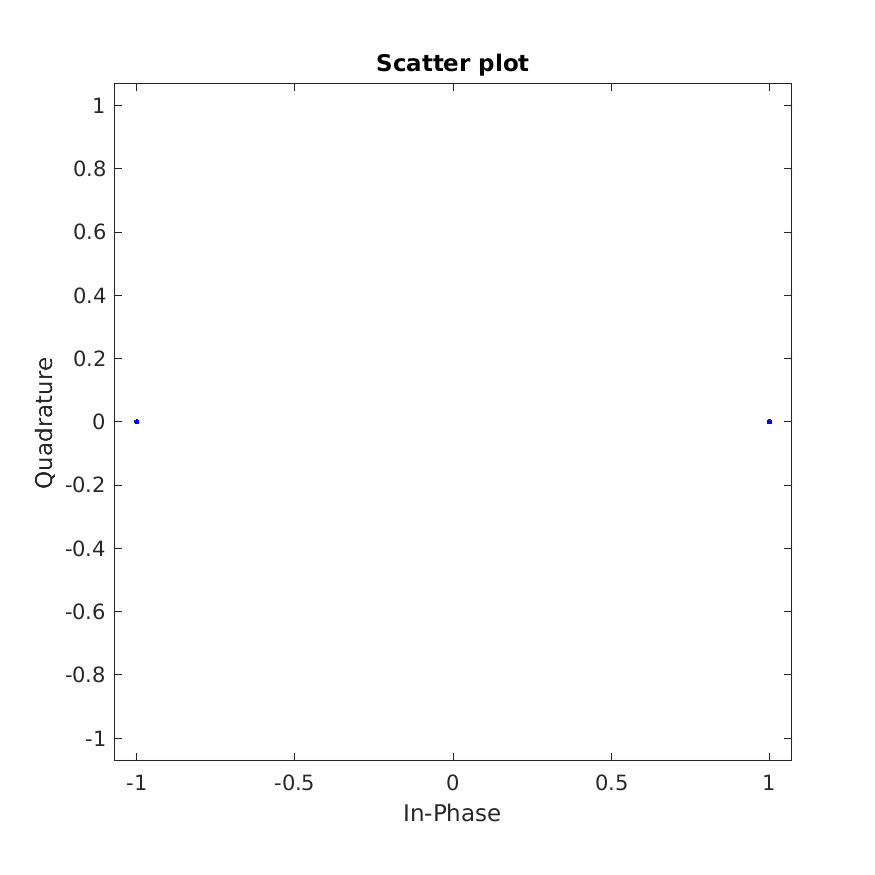
\includegraphics[scale=0.4]{lab6/figures/figure_0.png}
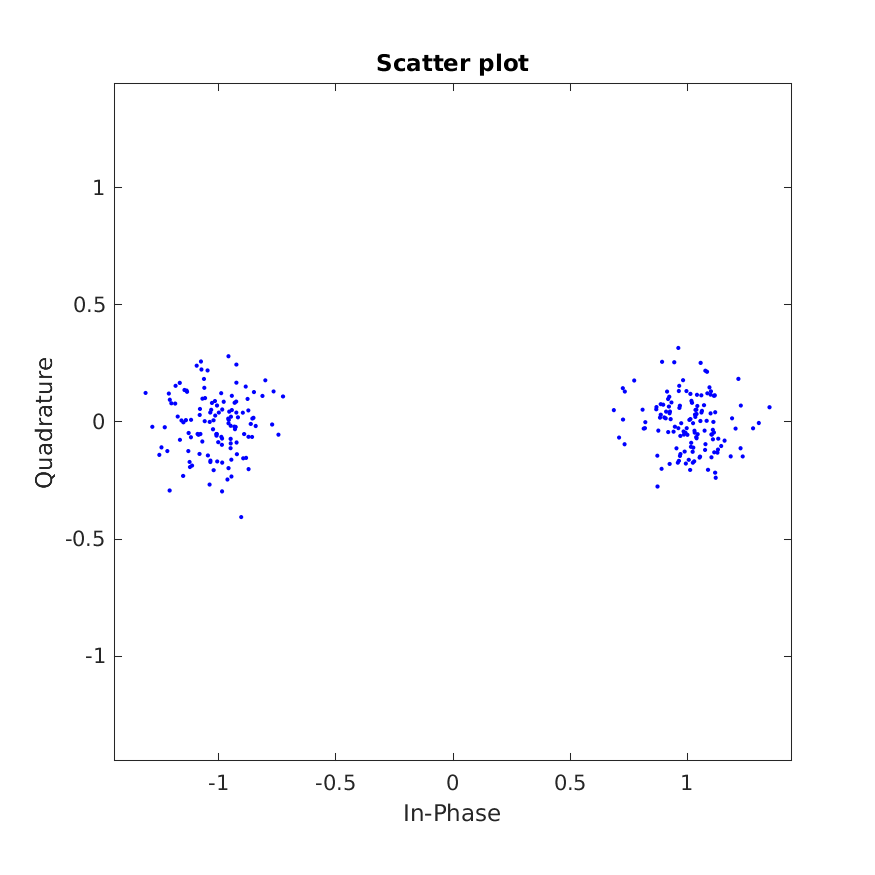
\includegraphics[scale=0.4]{lab6/figures/figure_1.png}\\
Число ошибочных символов: 0, вероятность ошибки на символ: 0.
\subsection{PSK}
Генерируем случайное сообщение, получаем сигнал от двоичного фазового модулятора и сигнальное созвездие $PSK$:
\lstinputlisting[language=Matlab]{lab6/psk.m}\\
Полученное сигнальное созвездие и зашумлённое сигнальное созвездие $PSK$:\\
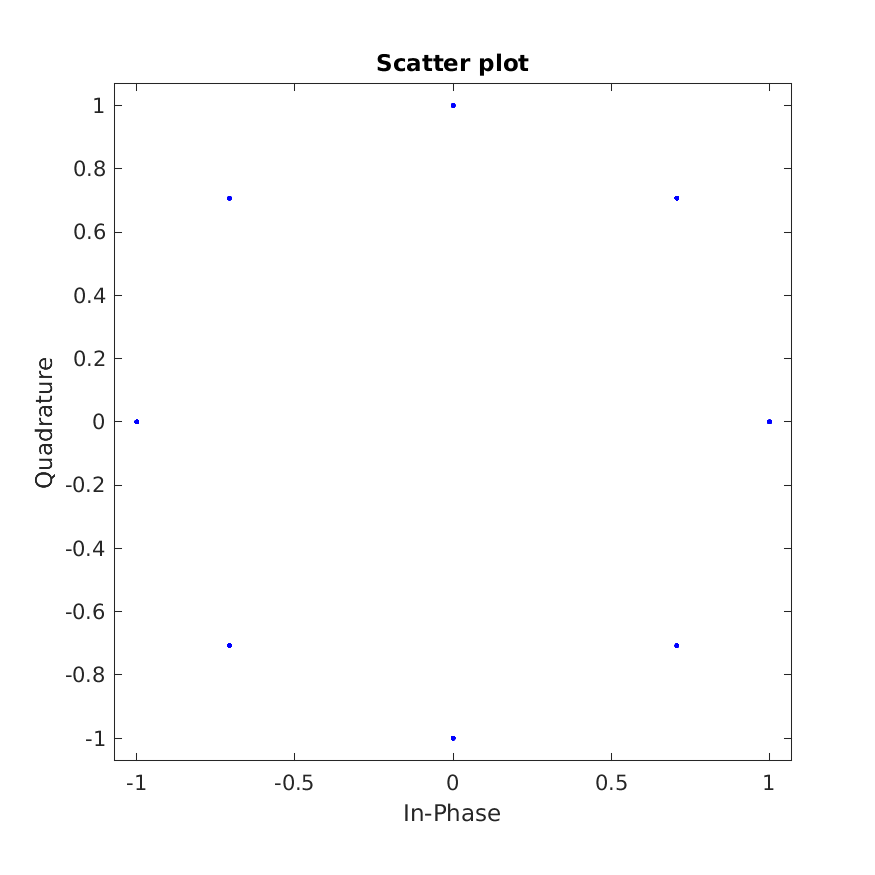
\includegraphics[scale=0.4]{lab6/figures/figure_2.png}
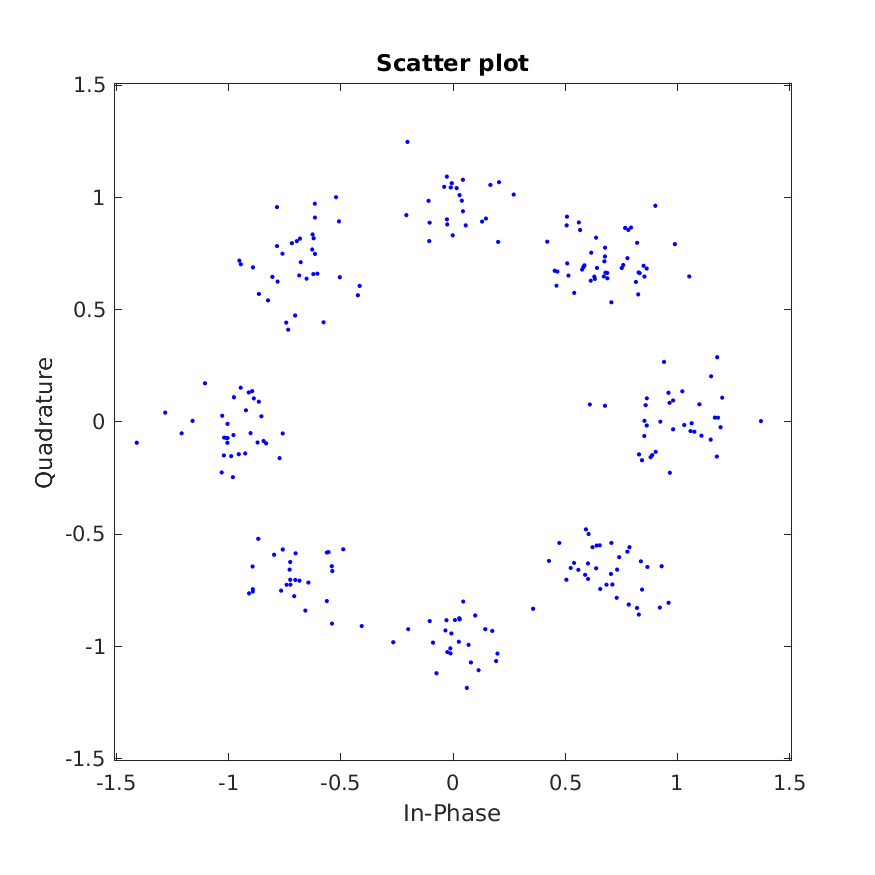
\includegraphics[scale=0.4]{lab6/figures/figure_3.png}\\
Число ошибочных символов: 4, вероятность ошибки на символ: 0.0156.
\subsection{OQPSK}
Генерируем случайное сообщение, получаем сигнал от двоичного фазового модулятора и сигнальное созвездие $OQPSK$:
\lstinputlisting[language=Matlab]{lab6/oqpsk.m}\\
Полученное сигнальное созвездие и зашумлённое сигнальное созвездие $OQPSK$:\\
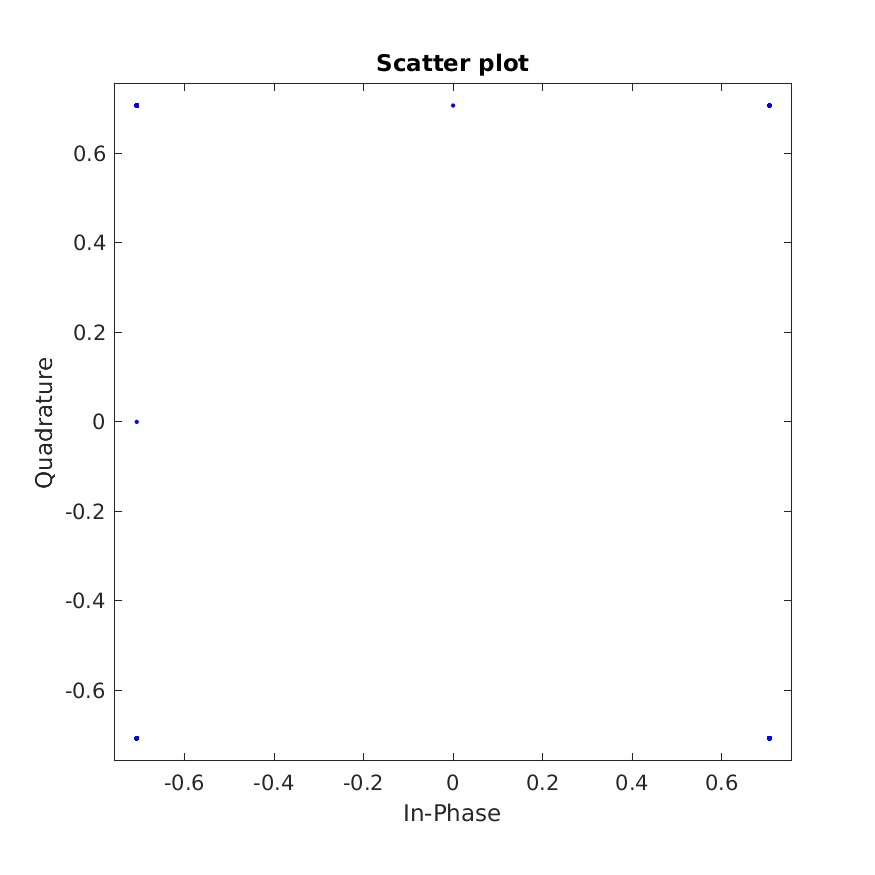
\includegraphics[scale=0.4]{lab6/figures/figure_4.png}
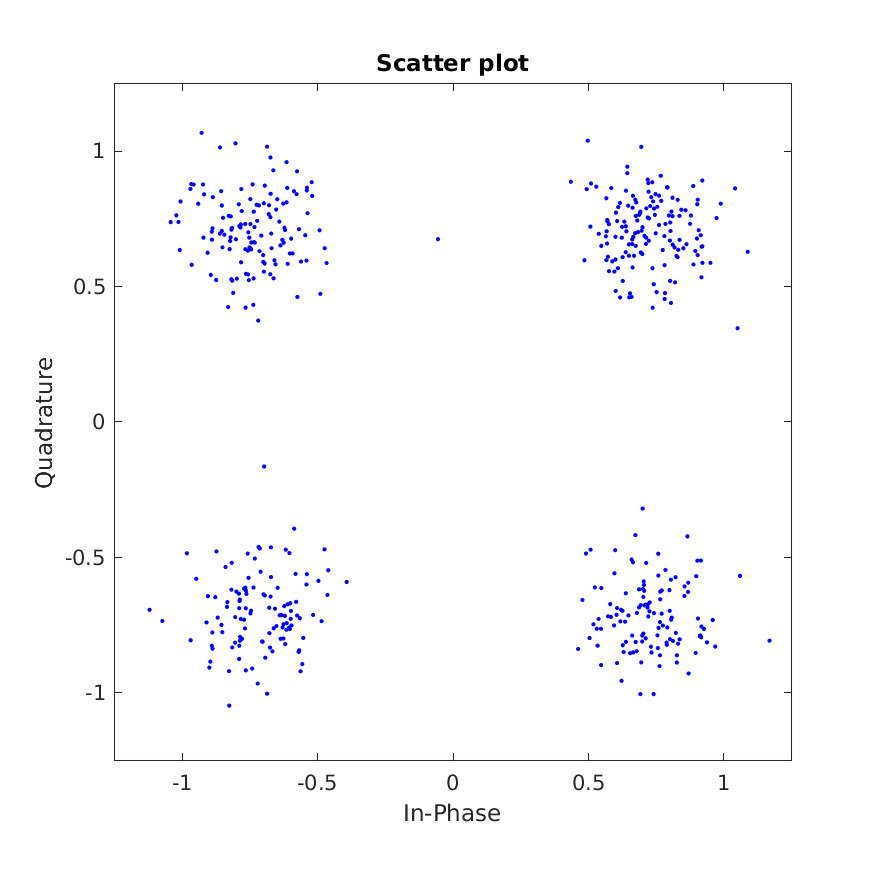
\includegraphics[scale=0.4]{lab6/figures/figure_5.png}\\
Число ошибочных символов: 0, вероятность ошибки на символ: 0.
\subsection{genQAM}
Генерируем случайное сообщение, получаем сигнал от двоичного фазового модулятора и получаем сигнальное созвездие $genQAM$:
\lstinputlisting[language=Matlab]{lab6/genqam.m}\\
Полученное сигнальное созвездие и зашумлённое сигнальное созвездие $genQAM$:\\
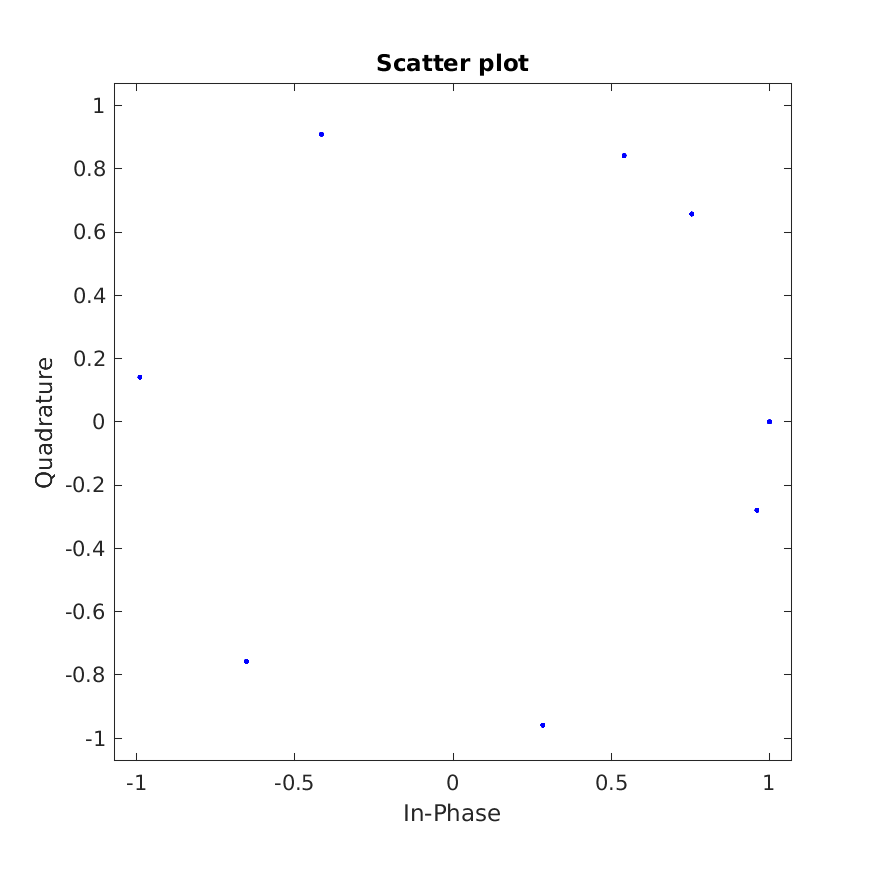
\includegraphics[scale=0.4]{lab6/figures/figure_6.png}
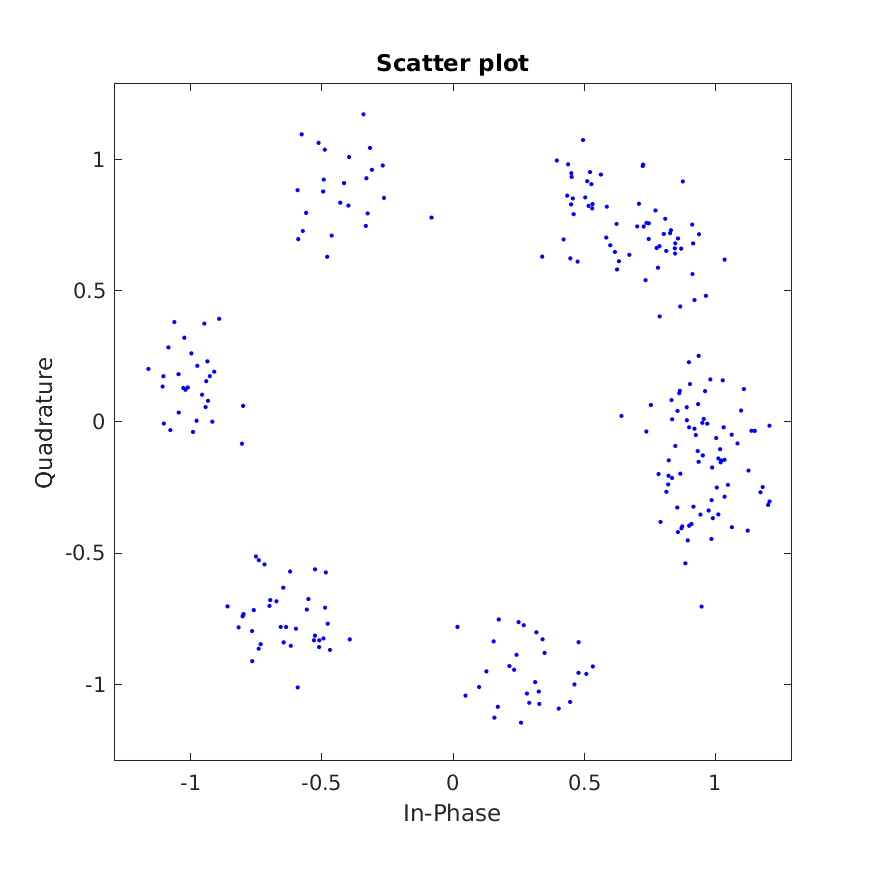
\includegraphics[scale=0.4]{lab6/figures/figure_7.png}\\
Число ошибочных символов: 13, вероятность ошибки на символ: 0.0508.
\subsection{MSK}
Генерируем случайное сообщение, получаем сигнал от двоичного фазового модулятора и сигнальное созвездие $MSK$:
\lstinputlisting[language=Matlab]{lab6/msk.m}\\
Полученное сигнальное созвездие и зашумлённое сигнальное созвездие $MSK$:\\
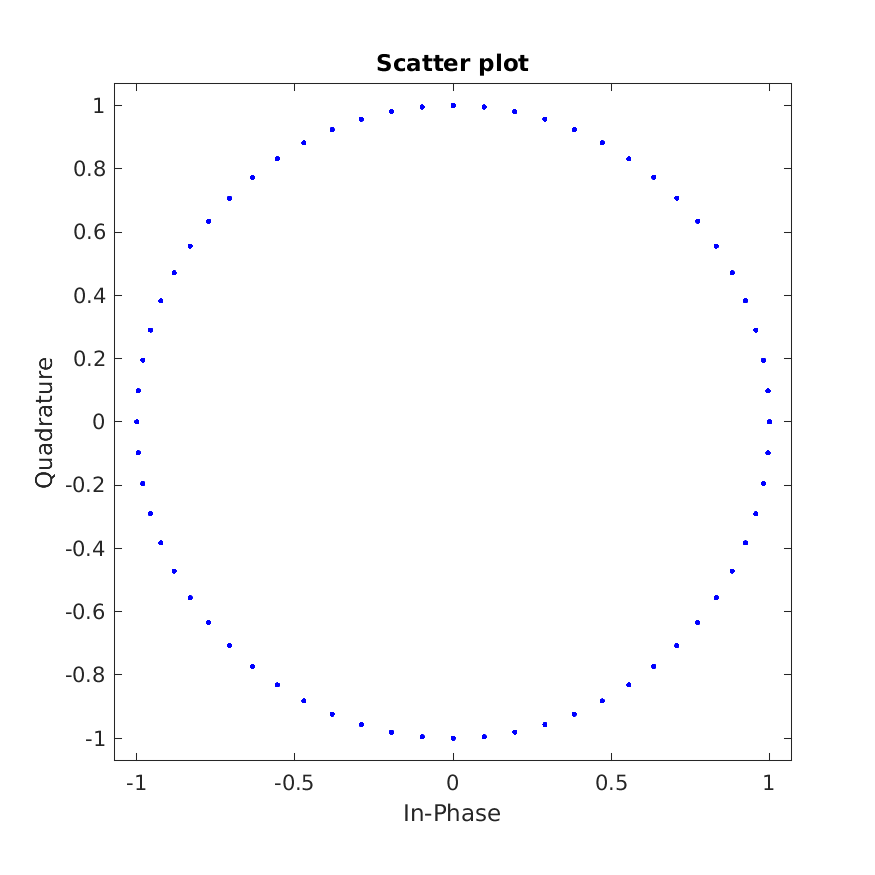
\includegraphics[scale=0.4]{lab6/figures/figure_8.png}
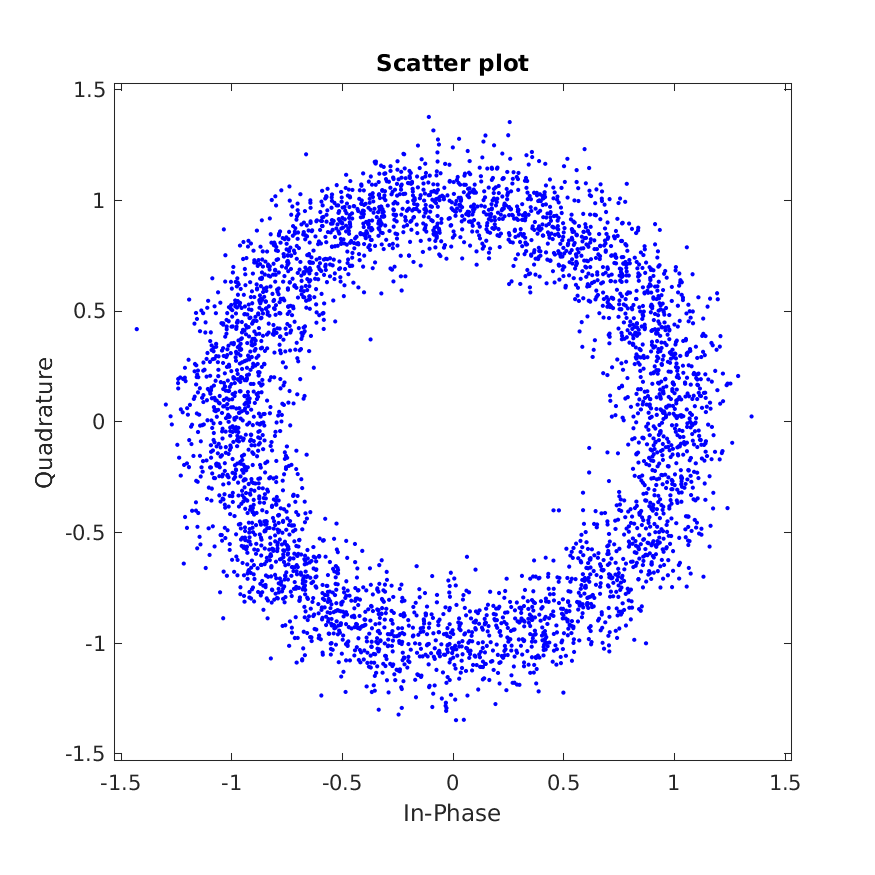
\includegraphics[scale=0.4]{lab6/figures/figure_9.png}\\
Число ошибочных символов: 0, вероятность ошибки на символ: 0.
\subsection{FSK}
Генерируем случайное сообщение, получаем сигнал от двоичного фазового модулятора и сигнальное созвездие $FSK$:
\lstinputlisting[language=Matlab]{lab6/fsk.m}\\
Полученное сигнальное созвездие и зашумлённое сигнальное созвездие $FSK$:\\
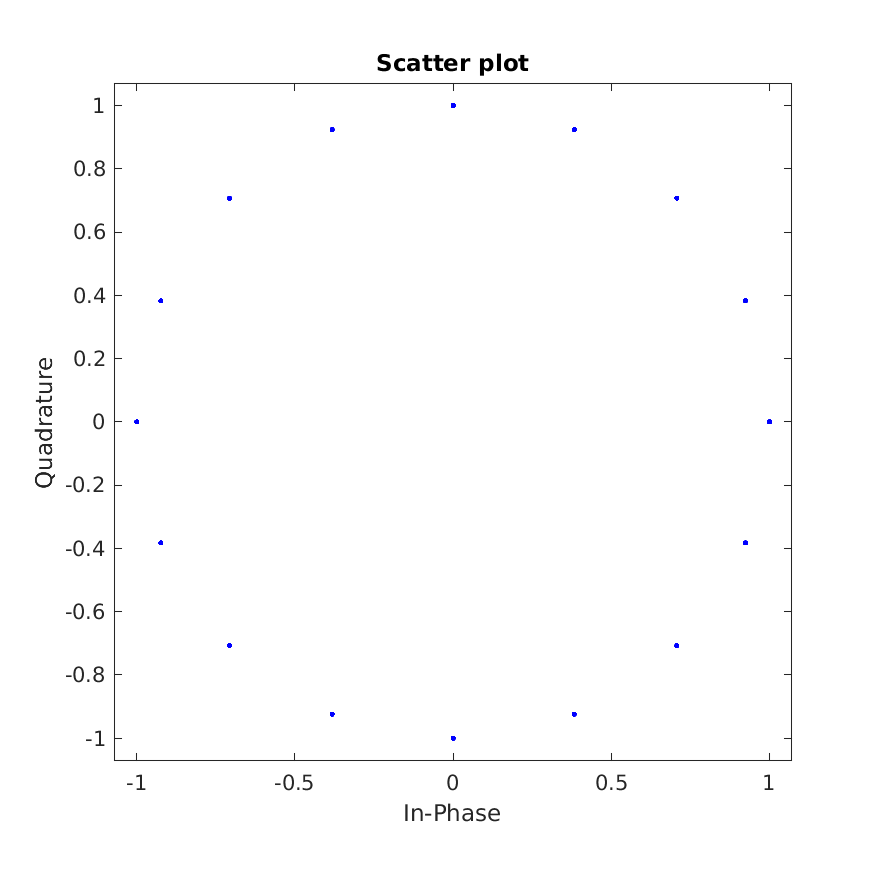
\includegraphics[scale=0.4]{lab6/figures/figure_10.png}
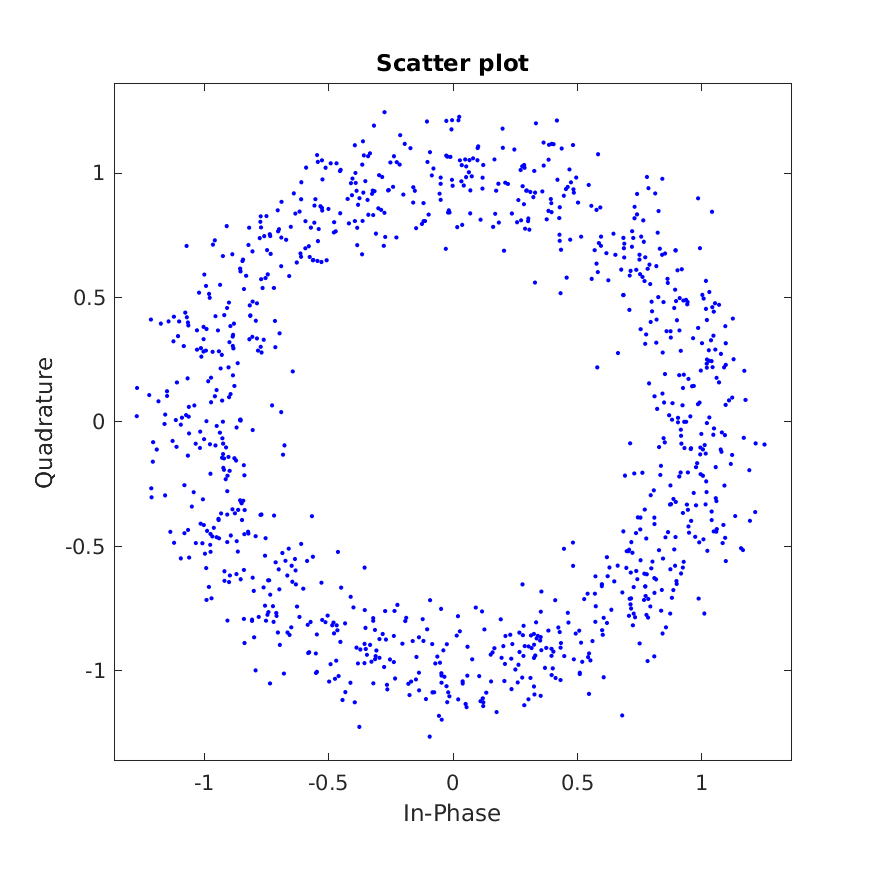
\includegraphics[scale=0.4]{lab6/figures/figure_11.png}\\
Число ошибочных символов: 0, вероятность ошибки на символ: 0.
\section{Сравнение методов модуляции}
Сравним изученные выше методы модуляции. Отобразим на графике зависимость SNR от вероятности ошибки для каждого рассмотренного метода модуляции.
Результат сравнения:\\
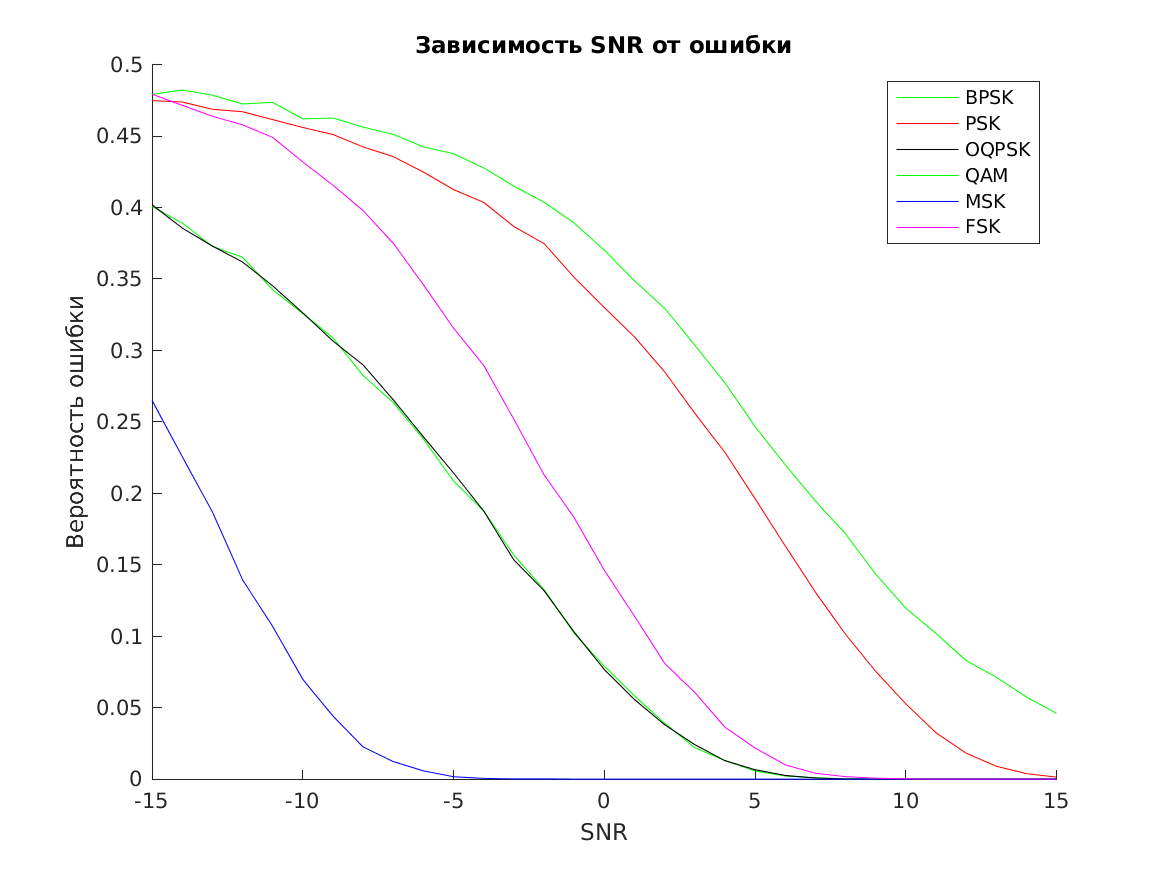
\includegraphics[scale=0.7]{lab6/figures/figure_12.png}\\
\section{Вывод}
Цифровая модуляция - это процесс преобразования цифровых символов в сигналы с характеристиками канала. При низкочастотной модуляции эти сигналы обычно имеют вид импульсов заданной формы. В случае полосовой модуляции импульсы заданной формы модулируют синусоиду, насываемую несущей; для радиопередачи на нужное расстояние
несущая преобразуется в электромагнитное поле.\\

В даной лабораторной работе были рассмотрены различные виды цифровой модуляции. Тип цифровой модуляции выбирается в зависимости от требований к скорости передачи и помехозащищенности. Самой надежной считается квадратурная манипуляция, так как информацию можно подавать сразу по двум параметрам. Для повцышения скорости передачи могут быть использованы PSK или QAM с большим количеством точек, что в свою очередь негативно скажется на помехоустойчивости вследствие их близкого расположения друг относительно друга на сигнальном созвездии. Число бит, передаваемых одним состоянием, определяется как log2N, где N - уровень модуляции. Таким образом, чем выше уровень модуляции, тем больше данных мы можем передать (или потерять) за единицу времени.
\end{document}